\documentclass[14pt]{article}
\usepackage[margin=0.8in]{geometry}
\usepackage{fancyvrb}
\usepackage{graphicx}
\usepackage{subcaption}
\usepackage{hyperref}
\hypersetup{
	colorlinks=true, %set true if you want colored links
	linkcolor=black, %choose some color if you want links to stand out
	urlcolor=blue
}
\graphicspath{ {./images/} }

\setlength{\parindent}{0pt}

\title{CCTF - Report}
\date{18/11/2020}
\author{Nail Dupre, Guadagnini Giovanni, Enrico Micheli, Davide Piva}

\begin{document}
	
\maketitle
	
\tableofcontents
\newpage
\section{Overview}
This report concern the two cctf laboratories:
\begin{itemize}
	\item \textbf{Resilient CCTF}: During this ctf the main purposes were to both to attack and defend a HTTP server against different type of attacks.
	\item \textbf{Secure CCTF}: 
\end{itemize}

\section{Resilient Server}
As already introduced in the Overview section this cctf was targeted to both offend and defend an HTTP server. Each group during the experience have access to two Deterlab experiments, in the first experiment the group will act as defenders (Blue Team) and in the second as attackers (Red Team).

\begin{figure}[!h]
	\centering
	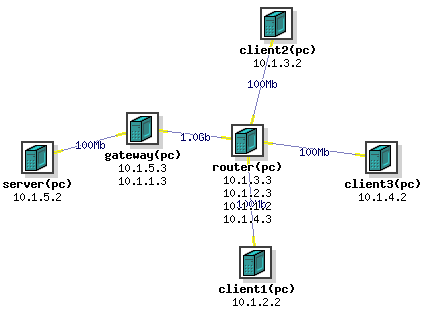
\includegraphics[width=8cm,height=6cm]{ResilientServerTopology}
	\caption{Topology of the Resilient Server CCTF.}
\end{figure}

This image describe the topology of the laboratory, that can be subdiveded in 3 areas:
\begin{itemize}
	\item \textbf{Clients machines}: These machines will be used from the attacker team. One of the three computer will be used as the genuine client that will try to reach the server with legitimate requests with a maximium rate of 1 request every second, the attackers will use the other two machines to attack the server in order to try to deny service to the genuine client.
	
	\item \textbf{Server and Gateway}: This two machine will be used from the defender team, in the specific the server will be equipped with a webserver, that serve 10 html pages, and the gateway will be used to try to block eventual attacks.
	
	\item \textbf{Router}: This machine will connect the machines controlled from the two groups and will be used to count the score.
\end{itemize}

\textbf{Attention}: The link between router and gateway is different from all the other links. In the specific the link provide 1 gb of bandwidth and allows all the client connected to the router to send the maximum amount of data allowed from the 100 mb links, and this is very suitable to launch flood attacks.
\\
\\
During the ctf attackers earn a points when a genuine request from the client take more than 0.5 seconds to be received, and on the contrary the point is given to the defenders group if the request is received from the client before half a second is passed. 

\subsection{Dupre}

\subsection{Guadagnini}
During the cctf I started working by developing some milestones: 
\begin{itemize}
	\item monitor\_server.sh: This script perform a really fast check of the server status. By sending ping and curl requests the user can easily understand if the server it's slowed down by some attacks.
	
	\item analyze\_traffic.sh: This script will launch two python programs that by using tcpdump, thanks to system function of os python module, and finally by analyzing the collected traffic, will enable the user to know with precision how many packets have passed through the server and also which client are sending data. This script in the end wasn't used since a only python version of it seemed to be a bit faster.
	
	\item flood.sh: This is a simple script that act as a wrapper for the flooder program that will enable the user to flood an ip by specifying less parameter than usual.
	
	\item slow\_loris.py: I've dowloaded it from its repository and in the first moment I've only modified it to request for the page provided from the server.
\end{itemize}

I've concluded the intial part by writing the startup.sh script for both the blue and red part of the cctf:
\begin{itemize}
	\item Blue part startup.sh: The script by using ssh will automatically install the apache2 webserver, enable syn-cookies, create the pages in the /var/html/www folder, enable the slow-loris mitigation for apache2, setup the iptable rules and finally upload the milestone script in a shared folder /home/cctf. Also will configure the gateway by uploading the script and configure the iptables rules.
	
	\item Red part startup.sh: Through ssh will install all the packages needed and upload the script on a shared folder /home/cctf in all the clients.
\end{itemize}

\subsubsection{Strategies}
I've also developed the defense and attack strategy, that which over time have been modified according to the results obtained with the tests.

\paragraph{Defense strategy}
At first the defense was based on using the gateway to try to block unnecessary traffic, so I used a white list approach to allow only some kind of traffic to pass, in the specific:
\begin{itemize}
	\item All the traffic from loopback interface.
	\item All the traffic generated and directed to deterlab control network (192.168.0.0/16).
	\item All icmp traffic between gateway and server in the network 10.1.5.0/24.
	\item Icmp packet generated from the external network with a maximum rate of 1 icmp packet per second.
	\item The fragmented packet have been blocked to avoid fragmented attacks.
	\item All the incoming http traffic on port 80, and obviously the outgoing traffic generated from the server.
\end{itemize}
Finally I've specified the DROP default policy for all the iptables chain to block all the traffic that won't match with the inserted rule. This rules has been "installed" in client and server machines.
\\
To protect the server against slow DoS attacks I configured the libapache2-mod-qos that basically disables the keep-alive messages when the connections in the pool are running out.
\\
\\
I also tried to implement the protection using \textbf{Snort}, by using the installation script present in the Snort laboratory in the end I was able to try using it as defense. Snort in particular can be very useful for thwarting some attacks but it is very harmful for flooding attacks as being single thread it does not scale very well when the number of requests rises significantly. So using Snort I was able to stop slow\_loris attack very easily but when a simple Syn flood attack was initiated, the performance collapsed causing significant delays in delivering the packets to the server and therefore to the genuine client. For these reason I stopped using snort and looked for alternatives.
\\
\\
As a result of the attacks tested, the security measures implemented were able to defend the server from slow dos attack thanks to the apache module but were vulnerable to syn flood attack as a way to limit large amounts of traffic directed to the server had not yet been implemented.
\\
\\
From the beginning I understood that eventual rate limiters used with Snort or iptables were not suitable since they were cutting also the good traffic, so the solution to have a good defense is to inspect the big amount of traffic an hope to find some differences with the genuine packets. Fortunately I was able to find two iptables module named \textbf{match-hex} and \textbf{match-string} that by inspecting the content of the packets were able to cut traffic without compromising the genuine client requests.


\paragraph{Attack strategy}
While deveoping the defense strategy I was trying to find some way to beat it. This process of continuos modifications led me to modify the attacks so that with each "iteration" they were harder to distinguish than genuine traffic. 
\\
I formulated an assumption: if the attacks  we were using weren't working or were partially working, there was no need to send the maximum requests possible and accordingly to this fact the genuine traffic could be lowered to the minimum or just simply reduced to lower the number of points opponents were earning. So following this idea I've modified the genuine\_client.sh script to modify on-demand the number of request by reading a file created in the same folder, the rate could be easily modified using the script change\_rate.sh that remotely throug ssh was able to change the rate value saved on the file.
\\
\\
In order for the slow\_loris.py to be less recognizable, I've redefined the request header to be the same of curl and I've also randomized the field in the keep-alive requests in order to be more difficult to detect and block. I also thought of using 2 iptables rules that through NAT allow you to spoof the source ip address of the packets generated by the slow loris attack so that for those who defend it is difficult to understand where the traffic is coming from.
\\
\\
By observing the attacks I've suggested also to use scripts or packages that were able to modify the header fields in order to make the attacks as indistinguishable as possible from genuine traffic, for example by putting the window at the same value that is used by curl 64240 and using modified headers as for the slow loris attack.
\\
\\
Finally I've discovered that while using flood attacks a single process wasn't able to generate very big amount of traffic, for example over 70000 packet per second. So accordingly to the available bandwidth of the link I've suggested to lower down the number of "flood" packets generated from a single process in order to make sure to take advantage of the available bandwidth with multiple processes that were concurrently generating a reasonable number of packets.

\subsubsection{Final Evaluation}
During the two ctfs by analyzing the traffic an by using the match module of iptables I was able to cut a very big amount of traffic. 
\\
\\
During the first ctf, before the laboratory crashed I was able to cut off the a very big portion of the attack traffic and it seemed that the server was able to respond to genuine requests quickly.
\\
\\
Unfortunately in the second ctf the adversary team has been were very smart and managed to the defenses to be ultra-protective. In fact, using fragmented genuine requests, which were blocked by default by the gateway, they managed to score many points as the requests to the server never arrived. One of the methods I used to defend, in addition to blocking fragmented packets, was in fact to check that the DF (do not fragment) bit was not set to 1 in requests, this was typical in syn packets of flood attacks, but unfortunately it was also used from the other team to generate the genuine requests. Also by interspersing fragmented and non fragmanted genuine requests they managed to "protect" their attack as it seemed that the server was working correctly.


\subsection{Micheli}

\subsection{Piva}




\end{document}
